\documentclass[letterpaper, 10 pt, conference]{ieeeconf}  % Comment this line out if you need a4paper

%\documentclass[a4paper, 10pt, conference]{ieeeconf}      % Use this line for a4 paper

%\IEEEoverridecommandlockouts                              % This command is only needed if 
                                                          % you want to use the \thanks command

%\overrideIEEEmargins                                      % Needed to meet printer requirements.

% See the \addtolength command later in the file to balance the column lengths
% on the last page of the document

% The following packages can be found on http:\\www.ctan.org
\usepackage{graphics} % for pdf, bitmapped graphics files
\usepackage{epsfig} % for postscript graphics files
\usepackage{graphicx}
\usepackage{mathptmx} % assumes new font selection scheme installed
\usepackage{times} % assumes new font selection scheme installed
\usepackage{mathtools} % assumes amsmath package installed
\usepackage{amssymb}  % assumes amsmath package installed
\usepackage{tikz}
\usepackage{tabulary}
\newcommand{\hvec}{\overset{\rightharpoonup}}
\newcommand{\argmin}{\arg\!\min}
\newcommand{\norm}[1]{\left\lVert#1\right\rVert}
\newcommand{\quotes}[1]{``#1''}
\usetikzlibrary{calc,positioning, fit, arrows}
%\usepackage{biber}

\makeatletter
\newenvironment{tablehere}
  {\def\@captype{table}}
  {}

\newenvironment{figurehere}
  {\def\@captype{figure}}
  {}
\makeatother

\newcommand{\vect}[1]{\ensuremath{\mathbf{#1}}}
\newcommand{\mat}[1]{\ensuremath{\mathbf{#1}}}
\newcommand{\transpose}{\ensuremath{\mathsf{T}}}
\newcommand{\of}[1]{\ensuremath{\left(#1\right)}}

\title{\LARGE \bf
Multi-dimensional Optimization of Gasoline-fueled Variable Pitch Multirotor Aircraft
}


\author{Dallin Briggs, Gary Ellingson% <-this % stops a space
%\thanks{$^{1}$James Jackson is a MS student in the Department of Mechanical Engineering, Brigham Young University
%        {\tt\small jamesjackson@byu.edu}}%
%\thanks{$^{2}$Gary Ellingson is a MS student in the Department of Mechanical Engineering, Brigham Young University
%        {\tt\small gary.ellingson@byu.edu}}%
}


\begin{document}



\maketitle
\thispagestyle{empty}
\pagestyle{empty}


%%%%%%%%%%%%%%%%%%%%%%%%%%%%%%%%%%%%%%%%%%%%%%%%%%%%%%%%%%%%%%%%%%%%%%%%%%%%%%%%
\begin{abstract}

Currently, there are numerous multirotor UAVs that are available commercially and to consumers that are capable of lifting small payloads for an endurance of approximately 30 minutes. While these current multirotors are good for short endurance missions, there are few options for larger, higher payload capacity multirotors that are able to maintain flight for longer than an hour. This paper describes the optimization process used to develop a multirotor platform that maximizes the flight time of a gasoline-fueled multirotor UAV by varying several design variables related to the power required and the aerodynamics of the model.

\end{abstract}


%%%%%%%%%%%%%%%%%%%%%%%%%%%%%%%%%%%%%%%%%%%%%%%%%%%%%%%%%%%%%%%%%%%%%%%%%%%%%%%%
\section{INTRODUCTION}

\begin{itemize}
	\item{This paper looks at the why and how we are going to optimize a multirotor platform to maximize flight time.}
	\item{Talk about how the variables that are going to be optimized are rotor radius, fuel consumption rate, number of blade per rotor, number of rotors, rotor speed, and rotor pitch.}
	\item{Talk about why these variables were selected as design variables.}
	\item{Talk about some physical constraints, especially those imposed by the FAA.}
\end{itemize}


%%%%%%%%%%%%%%%%%%%%%%%%%%%%%%%%%%%%%%%%%%%%%%%%%%%%%%%%%%%%%%%%%%%%%%%%%%%%%%%
\section{Background}

Control of variable pitch multirotor aircraft was studied by Cutler \cite{Cutler2012}. There is a small, electric variable pitch quad commercially available \cite{stingray2016}.  There are also several hobbyist attempts at gas powered variable pitch quads \cite{diy2016}, \cite{hackaday2016}.

In our knowledge there has been no attempt to use a gas powered variable pitch quad to maximize the flight time for carrying a relatively large payload. 

There are many commercially available parts for a gas quad, including engines and variable pitch helicopter propellers. 

\section{MOTIVATION}

Nearly all commercial and consumer multirotor UAVs are powered by Lithium-Polymer batteries because of their high energy capacity to weight ratios. Although these batteries are very good and reliable, they still offer much lower specific energy ratios then that of liquid fuels such as gasoline. The average specific energy for Lithium-Polymer batteries is up to 0.95 MJ/kg, where gasoline is 46.4 MJ/kg. This means that a gasoline-fueled multirotor can potential fly much longer than a battery powered multirotor because it can carry more energy onboard. 

\begin{itemize}
	\item{Will talk more about some of the details using a gas engine entails in the paper.}
	\item{Speak briefly on the reasons for requiring variable pitch with a gas engine.} 
	\item{Speak on current platforms and capabilities and explain how this could fundamentally change the way multirotors are used in commercial applications, but not really for consumers.}
\end{itemize}


\begin{figurehere}
	\begin{center}
		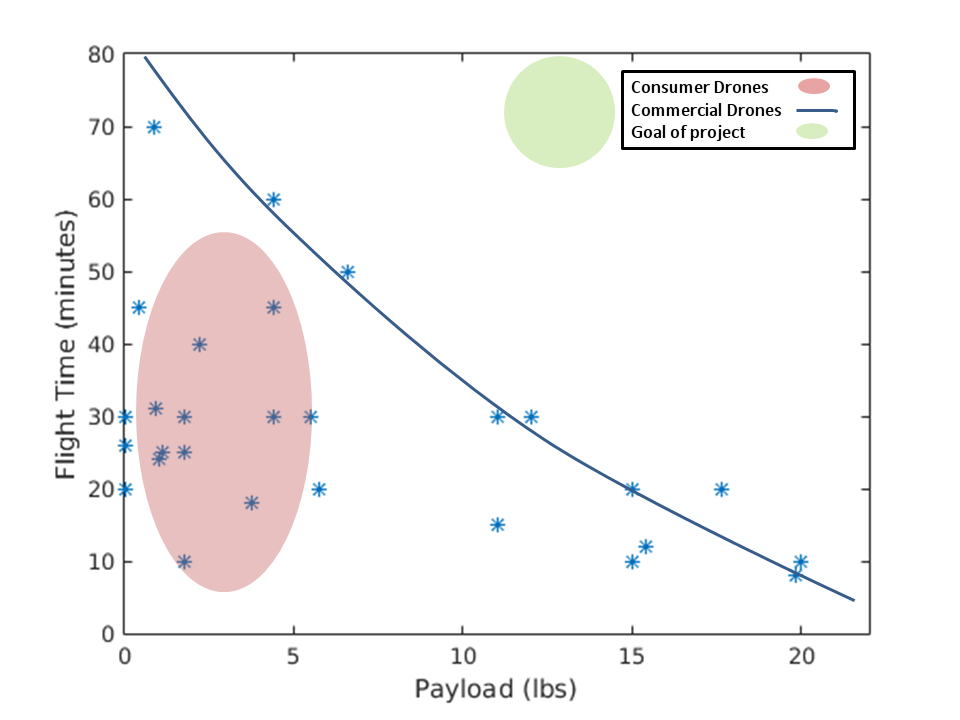
\includegraphics[width=.40\textwidth]{current_capabilities.png}
		\caption{\textit{Graphic showing current platforms and how our would be better.}}
		\label{current_cap}
	\end{center}
\end{figurehere}

	
%%%%%%%%%%%%%%%%%%%%%%%%%%%%%%%%%%%%%%%%%%%%%%%%%%%%%%%%%%%%%%%%%%%%%%%%%%%%%%%%%%
\section{METHODS}

Because the quad is going to be build using commercially available off-the-shelf parts the optimization must be closely based on reality.  This means we only can pick the size of engine that we are going to use.  All the other data about the engine (mass, maximum power, etc.) have to be a function of displacement size.  We collected data about popular two stroke RC aircraft engines from several sources to produce the below plots. 

\begin{figurehere}
	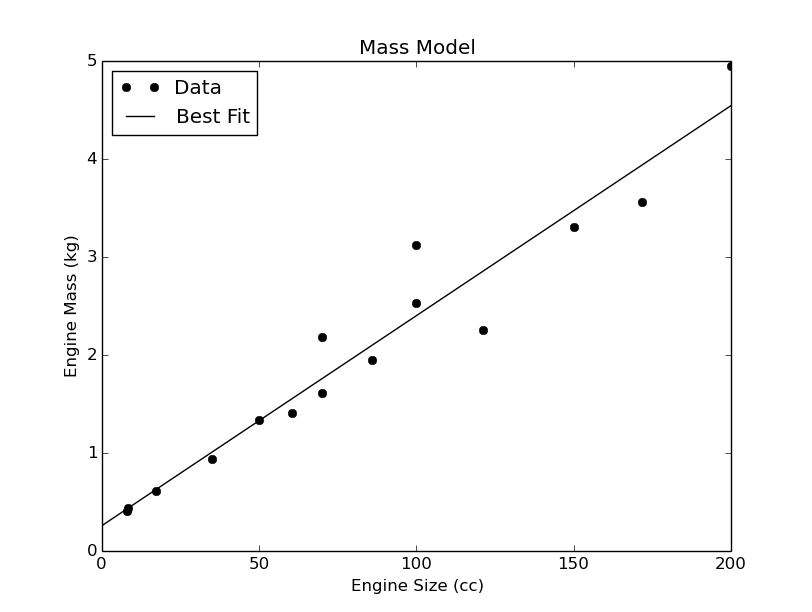
\includegraphics[width=0.5\textwidth]{mass.png}
	\caption{Stand in figure showing the data used to obtain the empirical based surrogate model of engine mass as a function of displacement size.}
		\label{fig:mass}
\end{figurehere}

\begin{figurehere}
	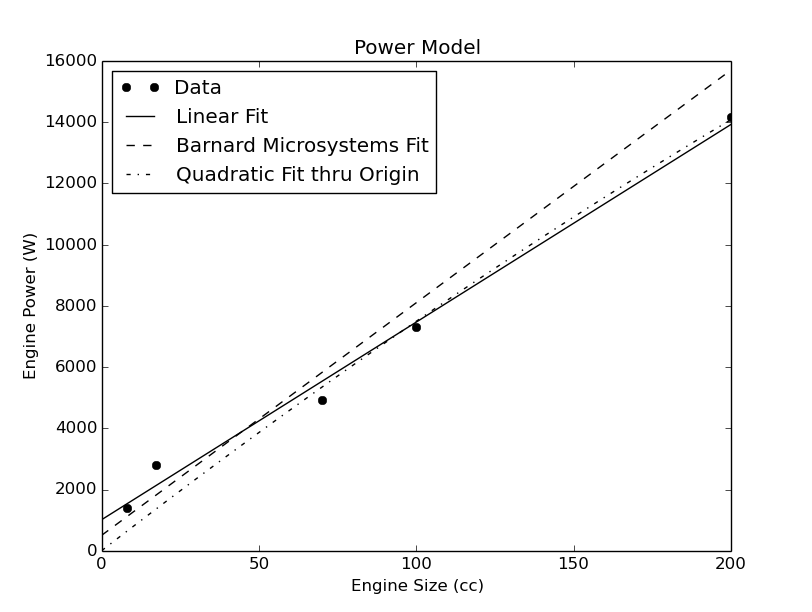
\includegraphics[width=0.5\textwidth]{max_power.png}
	\caption{Stand in figure showing the data used to obtain the empirical based surrogate model of engine maximum power as a function of displacement size.}
		\label{fig:power}
\end{figurehere}

The engine efficiency (friction and heat transfer losses), however, is a function of power capability of the engine (max power) and the power engine is required to produce.  For this we will need a better model.  \textit{We are still working on this. Since efficiency numbers for RC engines aren't publicly available, we need a scientific model.  For now we just assume a constant efficiency. We plan to work on this in the future.} 

Although the off-the-shelf constraint also applies to choosing the rotor parameters, continuous variables approximating the rotor specs are used and then analyzed as follows. 

\subsection{Aerodynamics}

Much of the work done in the methodology of optimizing flight time was to find adequate models for the thrust, torque, and power required from the main rotor disks. Since each rotor will be designed using small-scale helicopter components that consist of variable-pitch rotors that have no twist, a simplified helicopter rotor aerodynamic model should be sufficient for these calculations. 

Many of the existing aerodynamic models used in the aerospace industry to represent helicopter rotors are extremely complex and require specialized software tools (many of which are proprietary). High fidelity aerodynamic models generally require lots of computational power; so in order to focus on optimization methods rather than the complex aerodynamics of the system, several simplifications were made.

Combined differential blade element and momentum theory for nonuniform inflow was used to calculate the thrust and the torque differentially across each rotor blade \cite{bramwell2001bramwell}. The differential thrust is given by

\begin{equation}
	dT = \frac{1}{2} \rho a \Omega^2 r^2 (\theta - \phi) c \  dr,
	\label{thrust_eqn}
\end{equation}

where $\rho$ is the air density, \textit{a} is the lift-curve slope for the blade airfoil, $\Omega$ is the angular velocity of the rotors, \textit{r} is the radius of the annulus of the rotor being differentiated, $\theta$ is the blade pitch angle measured from the horizontal plane formed by the rotational disc of rotor blades, \textit{c} is the chord of the rotor, and $\phi = \tan^{-1}(U_p/U_T) $ is the inflow angle at the blade element. $U_P$ and $U_T$ are the components of air velocity relative to blade element perpendicular and tangential to the plane of rotation, respectively. The total thrust on each rotor is calculated by integrating equation \ref{thrust_eqn} across the rotor radius, \textit{R}. The total thrust for the multirotor can then be calculated by multiplying the blade thrust by the number of \textit{N} rotors. 

The differential torque for each rotor blade is given by

\begin{equation}
	dQ = \frac{1}{2} \rho \Omega^2 r^3 c (\delta + \phi C_L) \ dr,
	\label{torque_eqn}
\end{equation}

where $\delta$ is the local blade drag coefficient, and $C_L$ is the lift coefficient. The total torque for each blade and the multirotor can be found using the same method for calculating the thrust. 

The differential power produced by each rotor is given by 

\begin{equation}
	dP = dQ\Omega,
\end{equation}

and the total power can be calculated using the same method as thrust and torque. 


\section{OPTIMIZATION}

Our design variables are rotor radius, fuel consumption rate, number of blades per rotor, number of rotors, rotor speed, and rotor pitch. Rotor radius and number of blades per rotor, and number of rotors were chosen because this is an easy parameter to vary on multirotors due to the availability of numerous rotor blades available for small rotor aircraft. These variables also have a large influence on the flight time of the multirotor. Rotor speed and rotor pitch were chosen because these variables are easy to change on the physical system through selecting the proper gearing ratios. Fuel consumption rate seems like an odd variable for an optimizer because intuitively an optimizer would just minimize this value to maximize the flight time; however, fuel consumption rate is constrained by the size of engine required to produce the amount of power needed to provide enough lift for the multirotor. All of these design variables, however, have bound constraints that keep them in a reasonable space of commercially available parts/performance.

Setup the formal optimization problem
\begin{equation}
min. \quad f\of{x} = -t_{flight}\of{x}
\label{eq:objective}
\end{equation}
\begin{equation}
w.r.t. \quad x = [variables]^T
\label{eq:vars}
\end{equation}
\begin{equation}
s.t. \quad cons\of{x} \leq 0 
\label{eq:constrants}
\end{equation}

Flight time was calculated by 
\begin{equation}
	t_{flight} = K_{energy}*f_{capacity}/f_{rate}.
\end{equation}
Without constraints, the solution to maximizing flight time would be trivial to calculate as well as impossible to construct. Therefore to optimize the system we must use constraints that ensure the quad is feasible. The constrains are on the power produced by the engine ($P_{prod}$), power required by the prop ($P_{req}$), thrust produced by the prop ($T_{prod}$), lift required by the quad ($T_{req}$) and maximum power capabilities of the engine ($P_{max}$). Where $P_{preq} \leq P_{prod}$, $T_{req} \leq T_{prod}$, and $P_{prod} \leq P_{max}$.

We then will discuss the following:
\begin{itemize}
	\item{scaling of the design variables}
	\item{how we got gradients}
	\item{the optimization method that we utilized}
	\item{python vs matlab benefits and challenges}
\end{itemize}

Since we can only optimize for maximum flight time give a payload (parameter) we can further explore how the characteristics of a gas quad change as we optimize the flight time for different payloads. It may turn out that the optimal quad parameters change greatly as it is optimized for different payload.  In this case we could choose several payloads and optimize over all of then together. \textit{We will present these results with a figure and some discussion.}

\begin{figurehere}
	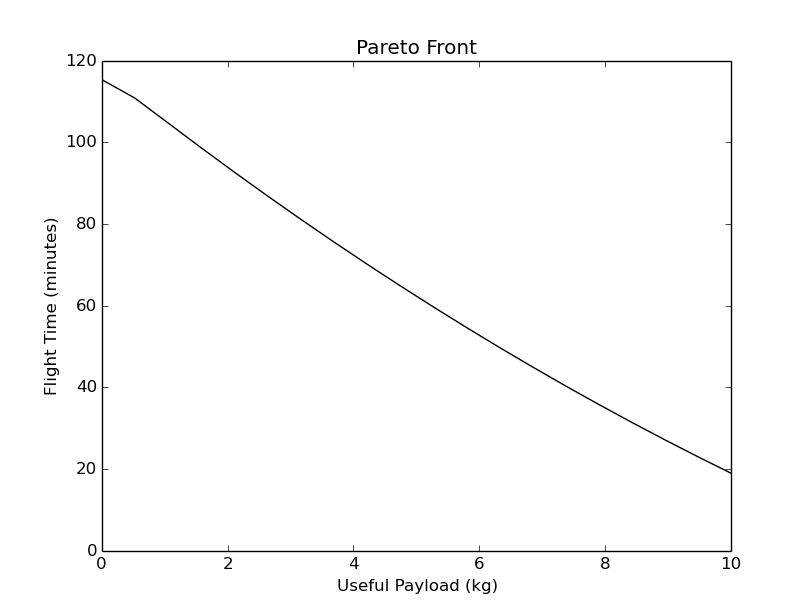
\includegraphics[width=0.5\textwidth]{pareto_front.png}
	\caption{Stand in figure showing optimal flight time as a function of payload.}
		\label{fig:payload}
\end{figurehere}

%Here we can do some discussion on constraint sensitivity - aerodynamics, engine efficiencies...

\section{RESULTS AND DISCUSSION}

We have found that the flight time of a gas-quad can be maximized by constructing with the following design.

\begin{tablehere}
\centering
\begin{tabulary}{0.5\textwidth}{|C|C|C|C|C|C|}
\hline
       & displacement & fuel rate & rotor radius & other \\ \hline
  & 100 & 30 & 250 & 150 \\ \hline
\end{tabulary}
\caption{Optimal design variables}
\label{table:fw_loop_rates}
\end{tablehere}


%%%%%%%%%%%%%%%%%%%%%%%%%%%%%%%%%%%%%%%%%%%%%%%%%%%%%%%%%%%%%%%%%%%%%%%%%%%%%%%%%%

\section{CONCLUSION}

lots of really good conclusions

%%%%%%%%%%%%%%%%%%%%%%%%%%%%%%%%%%%%%%%%%%%%%%%%%%%%%%%%%%%%%%%%%%%%%%%%%%%%%%%%
% \section*{APPENDIX}

% Appendixes should appear before the acknowledgment.

% \section*{ACKNOWLEDGMENT}

% Important people/organizations who made it possible


%%%%%%%%%%%%%%%%%%%%%%%%%%%%%%%%%%%%%%%%%%%%%%%%%%%%%%%%%%%%%%%%%%%%%%%%%%%%%%%%

\bibliography{./library}
\bibliographystyle{ieeetr}



\end{document}


%%%%%%%%%%%%%%%%%%%%%%%%%%%%%%%%%%%%%%%%%%%%%%%%%%%%%%%%%%%%%%%%%%%%%%%%%%%%%

% SAVED STUFF






%new document




